\documentclass[ngerman,hyperref={pdfpagelabels=false}]{beamer}

% -----------------------------------------------------------------------------

\graphicspath{{images/}}

% -----------------------------------------------------------------------------

\usetheme{KIT}

\setbeamercovered{transparent}
%\setbeamertemplate{enumerate items}[ball]

\newenvironment<>{KITtestblock}[2][]
{\begin{KITcolblock}<#1>{#2}{KITblack15}{KITblack50}}
{\end{KITcolblock}}

\usepackage[ngerman,english]{babel}
\usepackage[utf8]{inputenc}
\usepackage[TS1,T1]{fontenc}
\usepackage{array}
\usepackage{multicol}
\usepackage[absolute,overlay]{textpos}
\usepackage{beamerKITdefs}
\usepackage{amsfonts}


\pdfpageattr {/Group << /S /Transparency /I true /CS /DeviceRGB>>}	%required to prevent color shifting withd transparent images


\title{Tutorium 17, \#1}
\subtitle{Max Göckel -- \textit{uzkns@kit.edu}}

\author[Max Göckel]{Max Göckel}
\institute{Institut für Theoretische Informatik - Grundbegriffe der Informatik}

\TitleImage[width=\titleimagewd,height=\titleimageht]{titel}

\KITinstitute{Institut f\"ur Theoretische Informatik}
\KITfaculty{Fakult\"at f\"ur Informatik}

% -----------------------------------------------------------------------------

\begin{document}
\setlength\textheight{7cm} %required for correct vertical alignment, if [t] is not used as documentclass parameter


% title frame
\begin{frame}
  \maketitle
\end{frame}

%Einleitung
\begin{frame}
  \frametitle{Grundbegriffe?}
  \begin{itemize}
	\item Cloud
	\item Industrie 4.0
	\item Apps
	\item Operating Systems
	\item Big Data
	\item Roboter
	\item Künstliche Intelligenz
  \end{itemize}

... später im Studium, aber nicht in GBI.
\end{frame}

\begin{frame}
  \frametitle{Grundbegriffe!}
  \begin{itemize}
	\item Mengen, Relationen, Abildungen
	\item Wörter, Sprachen, RegEx
	\item Graphen
	\item Turingmaschinen
	\item Logik
	\item Technische Informatik (CPU)
  \end{itemize}

... im nächsten halben Jahr.
\end{frame}


%Tut Sinn
\begin{frame}
  \frametitle{Wofür ist dieses Tutorium da?}
 Ein Tutorium ist \textbf{kein} Ersatz für die Vorlesung! \\
\
  \begin{itemize}
	\item ÜBs zurück
	\item Definitionen aus der VL wiederholen
	\begin{itemize}
		\item Etwas weniger "formal", dafür mit Erklärung
		\item Wichtig: \textbf{Nur} Stoff aus der VL gilt verbindlich!
	\end{itemize}
	\item Def. anhand von Beispielen erklären
	\item Gemeinsam Aufgaben rechnen
  \end{itemize}
  
\end{frame}


%GBI Orga
\begin{frame}
  \frametitle{Das Modul GBI}

\begin{description}
	\item[Übungsschein]\hfill \\
Bestanden ab 50 Prozent der erreichten Punkte in den ÜBs
	\item[Klausur]\hfill \\
08.03.2018 14-16 Uhr, keine Hilfsmittel, schriftlich
\end{description}
GBI ist nach §9 Abs. 1, SPO 2015 Informatik Bestandteil der Orientierungsprüfung
\begin{itemize}
	\item Übungsschein im ersten Semster versuchen, spätestens im dritten bestehen
	\item Klausur spätestens im zweiten Semster versuchen, spätestens im dritten bestehen (Teilnahme ohne Übungsschein möglich)
\end{itemize}

\textbf{Andere Studiengänge?} Mal so, mal so. Bei Fragen im Modulhandbuch nachschauen oder bei Fachschaft / Studiengangsservice erfragen.
\end{frame}


%Übungsblätter
\begin{frame}
  \frametitle{Übungsblätter}
  \begin{itemize}
	\item Ausgabe: Mittwochs, alle 2 Wochen im ILIAS
	\item Abgabe: Donnerstags 16 Uhr 2 Wochen später im GBI-Kasten im Infobau-UG
	\item Rückgabe: Hier im Tut, sonst im Lehrstuhl
	\item Bearbeitung \textbf{ALLEINE} und ohne Abschreiben, sonst wars das mit Übungsschein 
  \end{itemize}
\end{frame}


%Übungsblätter 2
\begin{frame}
  \frametitle{Übungsblätter}
Modalitäten:
  \begin{itemize}
	\item Handschriftlich, 1x getackert und mit Deckblatt abgeben
	\item \textbf{Wichtig}: Tutoriumsnummer (42) und Name/Mat.-Nr. nicht vergessen
	\item Erlaubte Farben: Alles dunkle, zB kein grün oder rot
	\item Rand zum korrigieren frei lassen (am besten auch etwas zwischen den Aufgaben)
	\item Aufgaben markieren, in richtiger Reihenfolge abgeben
	\item Wenn ich es nicht lesen kann, gibt es keine Punkte
  \end{itemize}
\end{frame}


%Hilfe
\begin{frame}
  \frametitle{Fragen?}
Fragen:
  \begin{itemize}
	\item Hier im Tut (dafür ist es da)
	\item Ins ILIAS (dann können andere auch die Lösung lesen)
	\item Orga / Spezielles: An Zenkel oder an Stüker; am besten per Mail mit Matrikelnummer
	\item Fachliches: Sprechstunde, ILIAS
  \end{itemize}

Inhalt:
  \begin{itemize}
	\item Klausuren, Folien, Skript, ÜBs: ILIAS
	\item Archiv: gbi.ira.uka.de (noch mehr Klausuren, alte ÜBs, ...)
	\item iTunesU, YouTube, DIVA
  \end{itemize}
\end{frame}


%Noch mehr Hilfe
\begin{frame}
  \frametitle{Es geht nicht mehr?}
Bei Problemen aller Art:
  \begin{itemize}
	\item ILIAS-Kurs
	\item Kommilitonen, Tutoren, FS, Mitarbeiter
	\item Sprechstunde beim Professor (Do., 13-14 Uhr; 50.20/R231)
	\item zib, Allgemeine Studienberatung in 11.30; bei Fragen rund ums Studium
	\item Psychotherapeutische Beratungsstelle, Rudolfstr. 20; 0721-933-4060
	\item Nightline Karlsruhe unter www.nightline-karlsruhe.de
	\item Telefonseelsorge unter 0800-111-0-111 oder 0800-111-0-222
  \end{itemize}

\end{frame}

\begin{frame}
Jetzt geht es los
\end{frame}

% Mengen
\begin{frame}
  \frametitle{Mengen}

 \heading{M = \{1, 2, 3, 3\}}
  \begin{itemize}
  \item Sammlung von "Dingen" (Zahlen, Buchstaben, Öfen, ...)
  \item Ohne feste Reihenfolge (M = \{3, 3, 1, 2\})
  \item Ohne Duplikate (M = \{1, 2, 3\})
  \item Kardinalität einer Menge ist die Anzahl der Elemente in der Menge
 	\begin{itemize}
		\item Duplikate werden ignoriert
		\item Schreibweise |M| = 3 = |\{1, 2, 3\}|
	\end{itemize}
  \item Leere Menge \{\} bzw. $\emptyset$ hat Kardinalität 0
  \end{itemize}
  
\end{frame}


% Mengen v. Mengen
\begin{frame}
  \frametitle{Sonderfall Mengen "aus Mengen"}


  \begin{itemize}
	\item M = \{1, 2, 3\},   N = \{4, 5, 6, 7\}
	\begin{itemize}
		\item |M| = 3,    |N| = 4
	\end{itemize}
	\item aber X = \{M, N\}
	\begin{itemize}
		\item |X| = 2
	\end{itemize}
	\item Y = $\emptyset$,    Z = \{ $\emptyset$ \},
	\begin{itemize}
		\item  |Y| = 0, aber |Z| = 1
	\end{itemize}
  \end{itemize}

\end{frame}

%Schnitt u. Vereinigung
\begin{frame}
  \frametitle{Schnitt, Vereinigung, Differenz}

M = \{1, 2, 3, 4, 5\},   N = \{4, 5, 6, 7, 8\}

\begin{itemize}
\item Schnitt: $M \cap N = \{ x | x \in M \wedge x \in N \}$
\item Vereinigung: $M \cup N = \{ x | x \in M \vee x \in N \}$
\item Differenz: $M \backslash N = \{ x \in M | x \notin N \}$
\end{itemize}

\end{frame} %--------------------------------------
\begin{frame}
  \frametitle{Schnitt, Vereinigung, Differenz}

M = \{1, 2, 3, 4, 5\},   N = \{4, 5, 6, 7, 8\}

\begin{itemize}
\item Schnitt: $M \cap N = \{ x | x \in M \wedge x \in N \}$
	\begin{itemize}
	\item Konkret: 4, 5
	\end{itemize}
\item Vereinigung: $M \cup N = \{ x | x \in M \vee x \in N \}$
	\begin{itemize}
	\item Konkret:1, 2, 3, 4, 5, 6, 7, 8, 9
	\end{itemize}
\item Differenz: $M \backslash N = \{ x \in M | x \notin N \}$
	\begin{itemize}
	\item Konkret:1, 2, 3
	\end{itemize}
\end{itemize}

\end{frame}


%Teilmengen
\begin{frame}
  \frametitle{Teilmenge}

M = \{1, 2, 3, 4, 5\}, O = \{2, 3\}

\begin{itemize}
\item Echte Teilmenge: $O \subset M = \{ x \in O | x \in M \}$
\item Unechte Teilm.: $O \subseteq M$ = wie "echte", aber zusätzlich noch O = M

\end{itemize}

\end{frame}

%Potenzmenge
\begin{frame}
  \frametitle{Potenzmenge}

M = \{1, 2, 3\}

\begin{itemize}
\item Potenzmenge $2^M$ enthält alle Teilmengen von M
\end{itemize}

\end{frame} %---------------------------------------------
\begin{frame}
  \frametitle{Potenzmenge}

M = \{1, 2, 3\}

\begin{itemize}
\item Potenzmenge $2^M$ enthält alle Teilmengen von M
	\begin{itemize}
	\item Konkret: \{ $\emptyset$, \{1\}, \{2\}, \{3\}, \{1, 2\}, \{1, 3\}, \{2, 3\}, \{1, 2, 3\} \}, |$2^M$| = 8
	\end{itemize}
\end{itemize}

\end{frame}

%Tupel
\begin{frame}
  \frametitle{Tupel}
Schreibweise: (2, 3 ,4) oder (A, B, C, D)

Ähnlich einer Menge, aber mit besonderen Eigenschaften

\begin{itemize}
\item Reihenfolge ist wichtig: (2, 3, 4) $\not=$ (4, 3, 2)
\item Duplikate möglich, aber fest: (2, 2) $\not=$ (2, 2, 2)
\item Tupel aus Mengen möglich: (\{1, 2\}, \{3, 4\}) = (\{2, 1\}, \{4, 3\}) $\not=$ (\{3, 4\}, \{1, 2\})
\item Leeres Tupel bzw. 0-Tupel: ( )
\end{itemize}

\end{frame}

%Kartesisches Produkt
\begin{frame}
  \frametitle{Kartesisches Produkt}

M = \{1, 2\}, N = \{A, B\}

M $\times$ N = $\{ (m, n) | m \in M, n \in N \}$ ergibt eine Menge aus Tupeln aus M und N \\
\ \\


\end{frame} %-----------------------------------------------
\begin{frame}
  \frametitle{Kartesisches Produkt}

M = \{1, 2\}, N = \{A, B\}

M $\times$ N = $\{ (m, n) | m \in M, n \in N \}$ ergibt eine Menge aus Tupeln aus M und N \\
\ \\
Konkret:
\begin{itemize}
\item M $\times$ N = \{ (1, A), (2, A), (1, B), (2, B) \}
\end{itemize}

\end{frame}

%Zahlenmengen
\begin{frame}
  \frametitle{Zahlenmengen}

\begin{itemize}
\item $\mathbb{N}_{+}$, natürliche, positive Zahlen --- \{1, 2, 3, ...\}
\item $\mathbb{N}_{0}$, natürliche Zahlen mit der 0 --- $\mathbb{N}_{+} \cup 0$
\item $\mathbb{Z}_{n}$, ganze Zahlen von 0 bis n --- n = 3 $\Rightarrow$ \{0, 1, 2, 3\}
\item $\mathbb{Z}$, ganze Zahlen --- \{..., -3, -2, -1, 0, 1, 2, 3, ...\}
\item $\mathbb{Q}$, rationale Zahlen --- $\{\frac{x}{y}| x, y \in \mathbb{Z}, y \not= 0\}$
\item $\mathbb{R}$, reele Zahlen --- \{..., -5, 0, 1.5, e, $\Pi$, 1000, ...\}
\item $\mathbb{C}$, ...nicht hier
\end{itemize}

\end{frame}

%Alphabete
\begin{frame}
  \frametitle{Alphabete}

Ein Alphabet ist eine \emph{endliche, nichtleere} Menge aus Zeichen / Symbolen. Was dabei ein Zeichen ist, ist nicht eingeschränkt.\\
\ \\
Beipielalphabete:
\begin{enumerate}
\item \{H, a, n, d, y\}
\item \{Handy\}
\item \{Ha, ndy\}
\end{enumerate}
Können alle "Handy" erstellen/schreiben
\end{frame}

%Pelationen
\begin{frame}
\frametitle{Relation}

Relation R $\subseteq$ A $\times$ B, also enthält R Tupel aus der Menge A $\times$ B.\\
Im Fall  R $\subseteq$ A $\times$ A heißt R \emph{"Relation auf A"}.

\end{frame}


%Aufgaben Relationen
\begin{frame}
\frametitle{Aufgaben}
Relation 1, "größer-gleich-Relation": A = \{1,2,4\}, R = $\{(a_1, a_2)$ | $a_1, a_2 \in A: a_1 \ge a_2\}$\\
\ \\
Relation 2, "Ungleich-Relation": A = \{1,2\}, B = \{2,3,4\}, R = $\{(a, b)$ | $a \in A, b \in B: a \not= b\}$\\
\ \\
Welche Tupel sind in der Relation drin?\\
\ \\
\textit{\{(2,1), (4,1), (4,2)\} bzw. \{(1,2), (1,3), (1,4), (2,3), (2,4)\} }
\end{frame}

%linkstotal, etc.
\begin{frame}
\frametitle{Eigenschaften von Relationen}

\begin{itemize}
\item linkstotal: $\forall a \in A \exists b \in B: (a,b) \in R$
\item rechtseindeutig: $\nexists a \in A: (\exists b_1, b_2 \in B, b_1 \not= b_2: (a, b_1) \in R \wedge (a, b_2) \in R)$
\item rechtstotal: $\forall b \in B \exists a \in A: (a,b) \in R$
\item linkseindeutig: $\forall (a_1, b_1), (a_2, b_2) \in R: a_1 \not= a_2 \Rightarrow b_1 \not= b_2$
\end{itemize}
\end{frame}

%linkstotal
\begin{frame}
\frametitle{Linkstotal}

linkstotal: $\forall a \in A \exists b \in B: (a,b) \in R$\\
\ \\
\begin{itemize}
\item In Worten: Jedes Element a aus A hat \emph{mindestens} ein Element b aus B als Partner.
\item Eselsbrücke: Die "totale" (also komplette) linke Menge (A) wird in R verwendet.
\item Voraussetzung für eine Funktion
\end{itemize}
\end{frame}

\begin{frame}
\frametitle{Linkstotal}

\begin{figure}[htbp] 
\centering
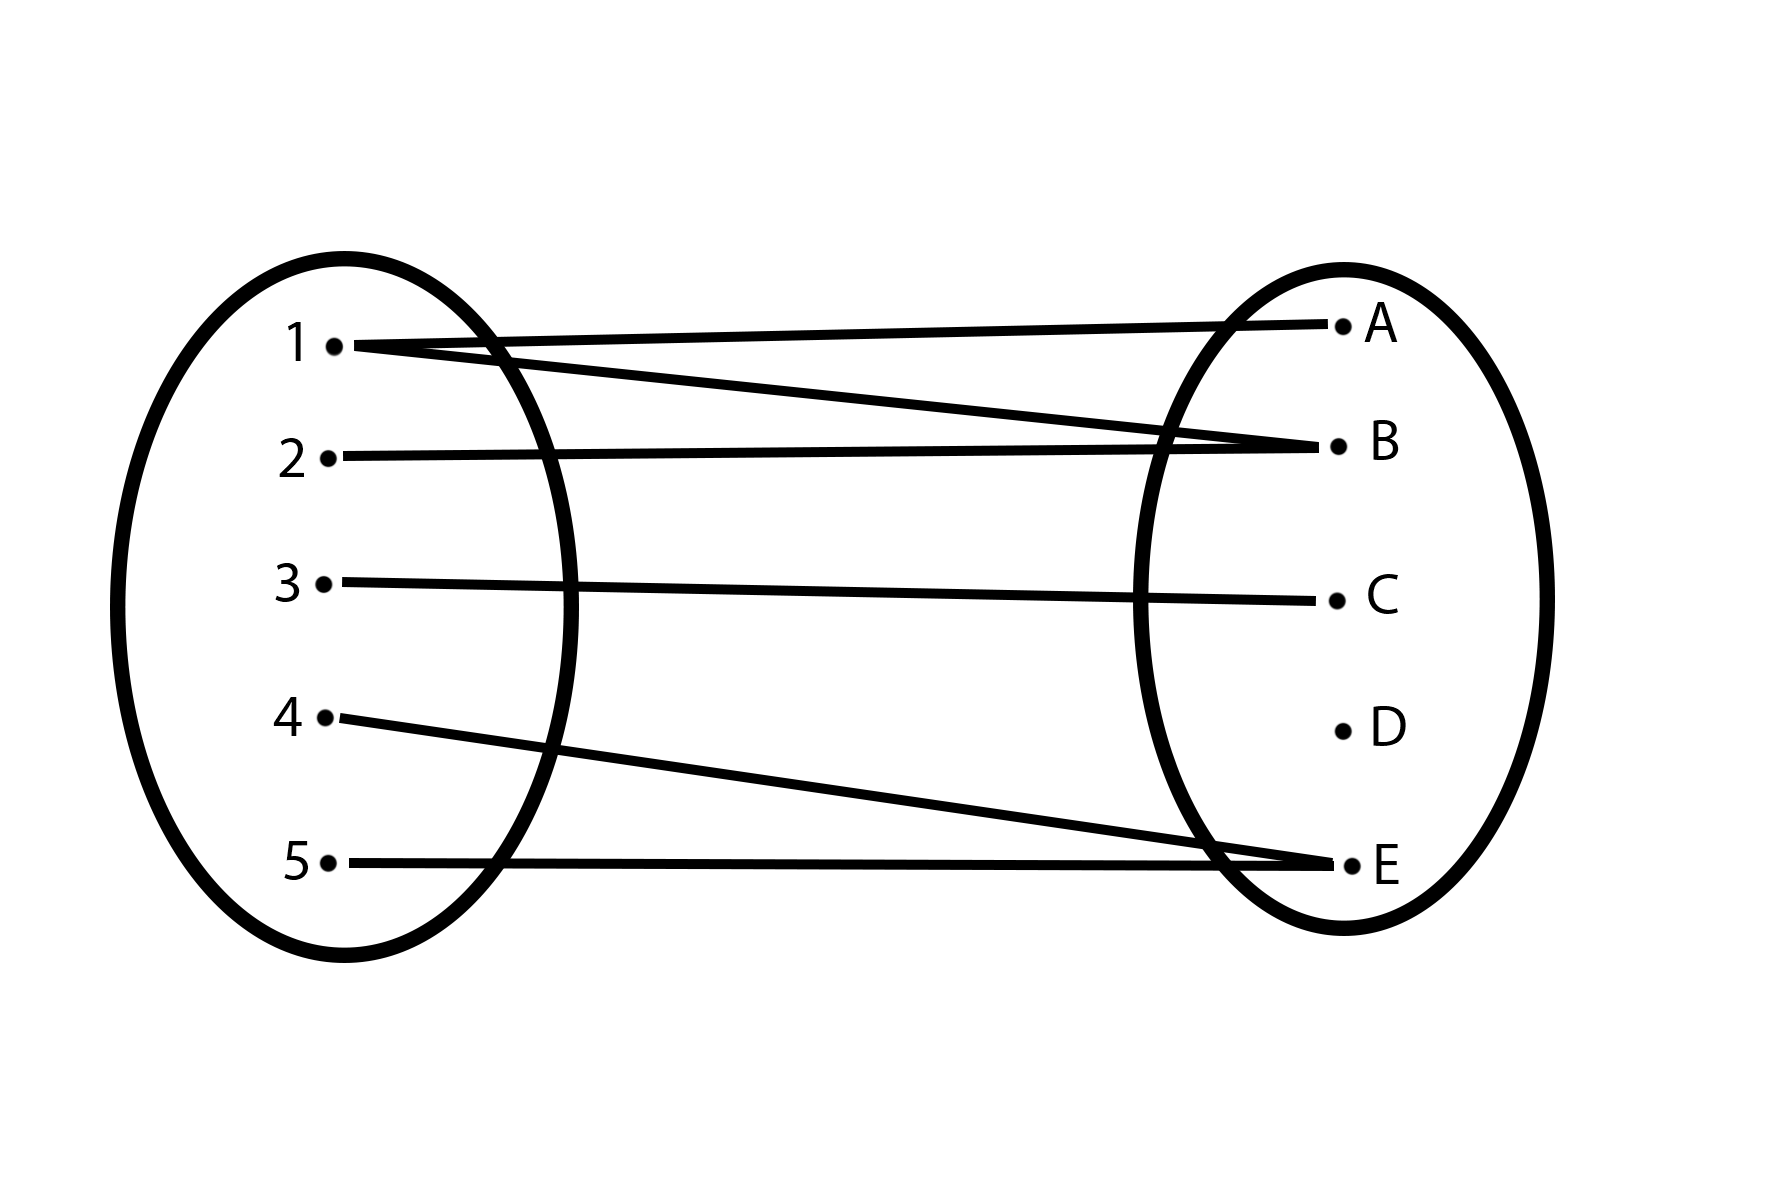
\includegraphics[width=0.7\textwidth]{images/linkstotal.png}
\caption{Linkstotal, Jedes linke Element hat min. ein rechtes Element}
\label{fig:Bild1}
\end{figure}
\end{frame}

%rechtstotal
\begin{frame}
\frametitle{Rechtstotal}

$\forall b \in B \exists a \in A: (a,b) \in R$\\
\ \\
\begin{itemize}
\item In Worten: Jedes Element b aus B hat \emph{mindestens} ein Element a aus A als Partner.
\item Eselsbrücke: Die "totale" (also komplette) rechte Menge (B) wird in R verwendet.
\item Auch surjektiv genannt
\end{itemize}
\end{frame}

\begin{frame}
\frametitle{Rechtstotal}

\begin{figure}[htbp] 
\centering
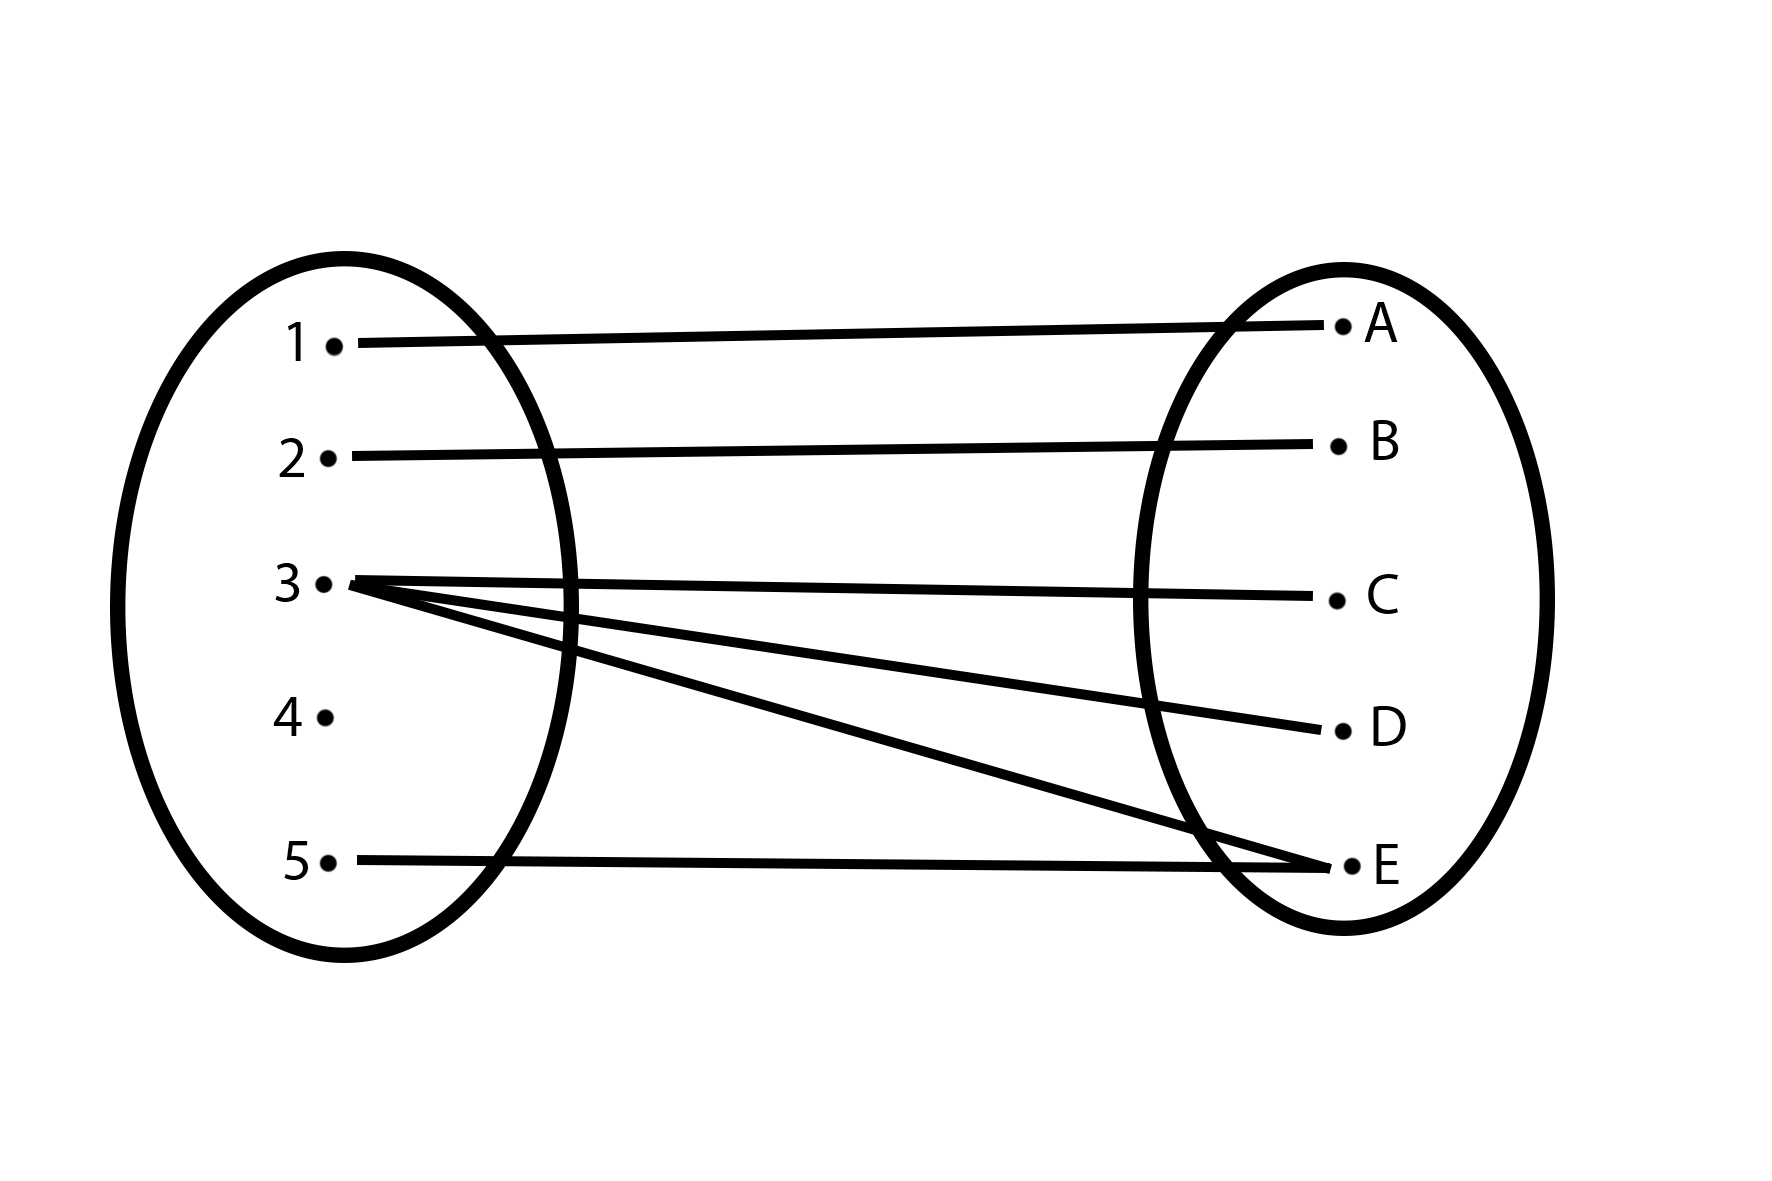
\includegraphics[width=0.7\textwidth]{images/rechtstotal.png}
\caption{Rechtstotal, Jedes rechte Element hat min. ein linkes Element}
\label{fig:Bild1}
\end{figure}
\end{frame}

%linkseindeutig
\begin{frame}
\frametitle{Linkseindeutig}

$\forall (a_1, b_1), (a_2, b_2) \in R: a_1 \not= a_2 \Rightarrow b_1 \not= b_2$\\
\ \\
\begin{itemize}
\item In Worten: Wenn ich zwei a aus A angucke und $a_1 \not= a_2$ so ist auch $b_1 \not= b_2$
\item Einfacher: Jedes Element b aus B hat \emph{höchstens} ein Element a aus A als Partner.
\item Eselsbrücke: Das linke Element ist zum rechten Element eindeutig.
\item Auch injektiv genannt
\end{itemize}
\end{frame}

\begin{frame}
\frametitle{Linkseindeutig}

\begin{figure}[htbp] 
\centering
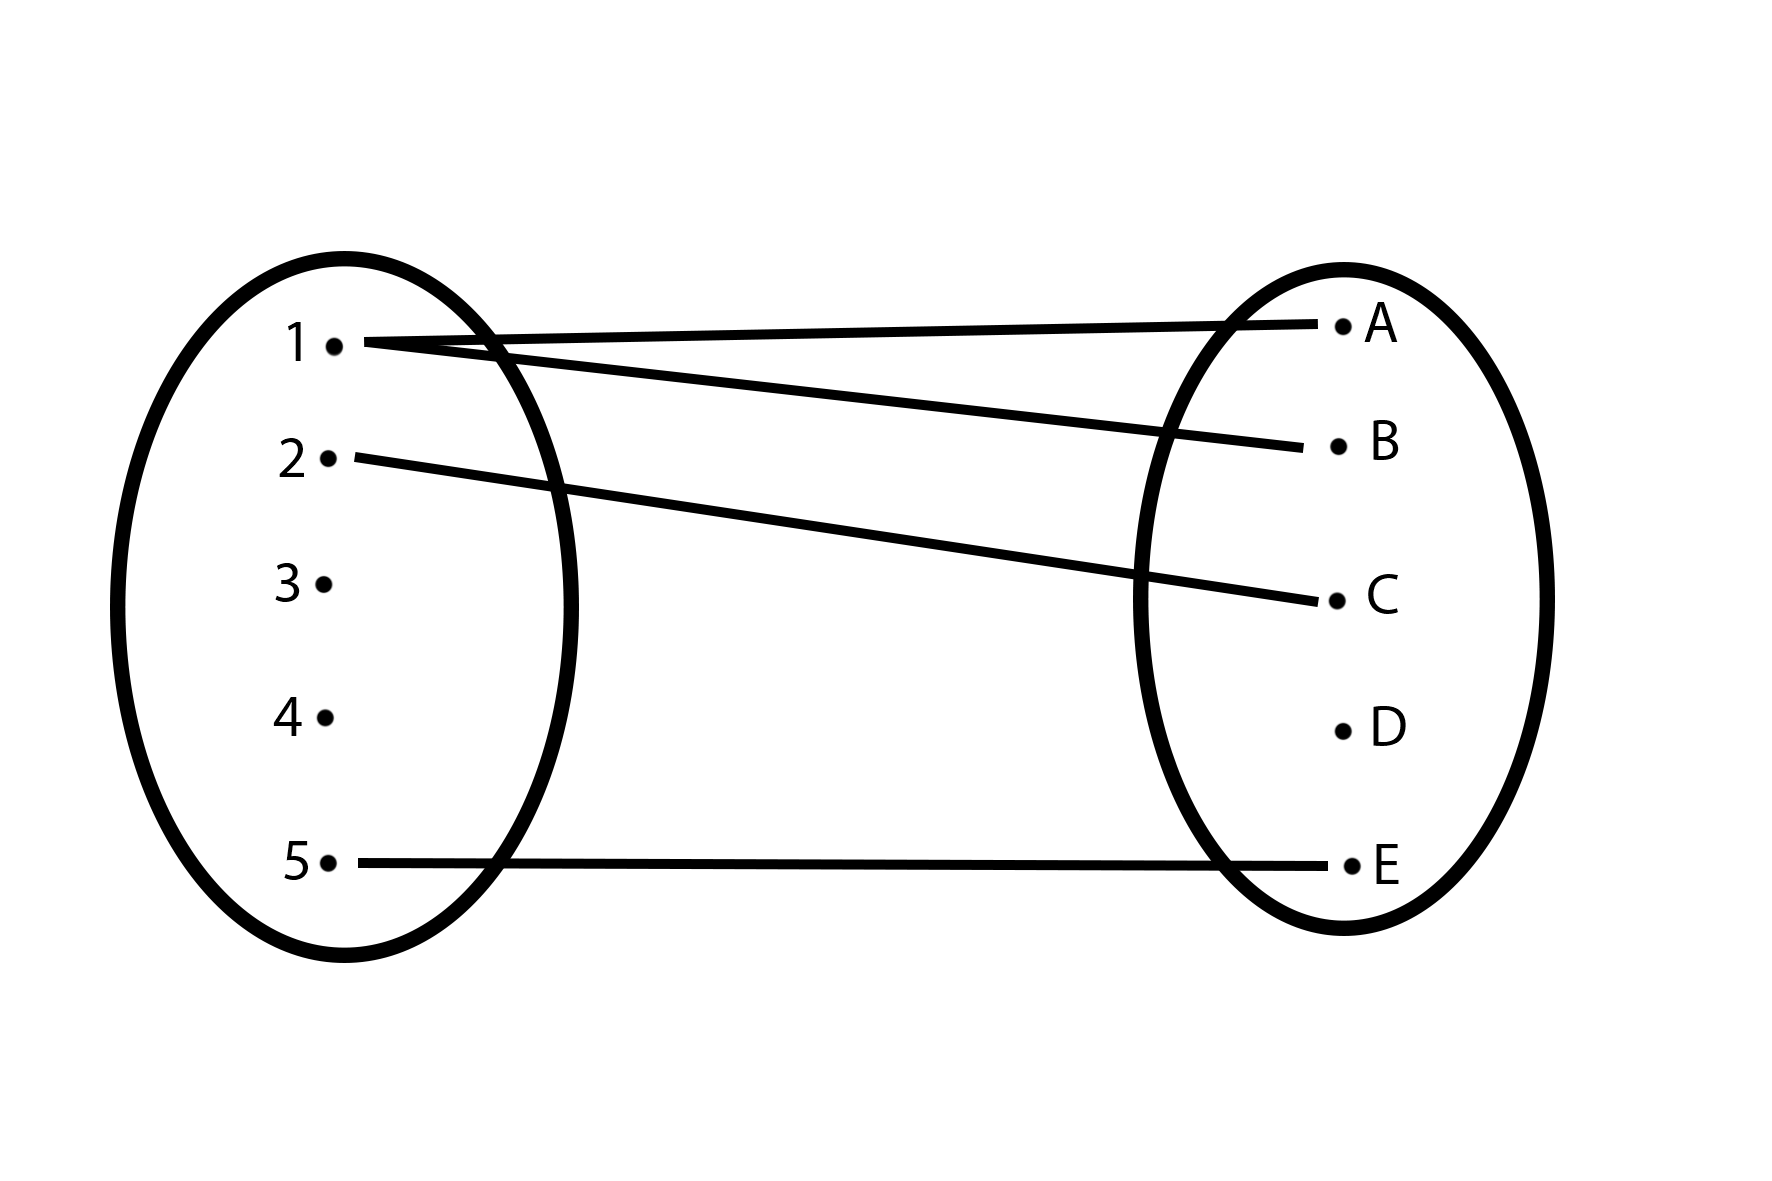
\includegraphics[width=0.7\textwidth]{images/linkseindeutig.png}
\caption{Linkseindeutig, Jedes rechte Element hat höchtens ein linkes Element}
\label{fig:Bild1}
\end{figure}
\end{frame}

%rechtseindeutig
\begin{frame}
\frametitle{Rechtseindeutig}

$\forall (a_1, b_1), (a_2, b_2) \in R: b_1 \not= b_2 \Rightarrow a_1 \not= a_2$\\
\ \\
\begin{itemize}
\item In Worten: Wenn ich zwei b aus B angucke und $b_1 \not= b_2$ so ist auch $a_1 \not= a_2$
\item Einfacher: Jedes Element a aus A hat \emph{höchstens} ein Element b aus B als Partner.
\item Eselsbrücke: Das rechte Element ist zum linken Element eindeutig.
\item Voraussetzung für eine Funktion
\end{itemize}
\end{frame}

\begin{frame}
\frametitle{Rechtseindeutig}

\begin{figure}[htbp] 
\centering
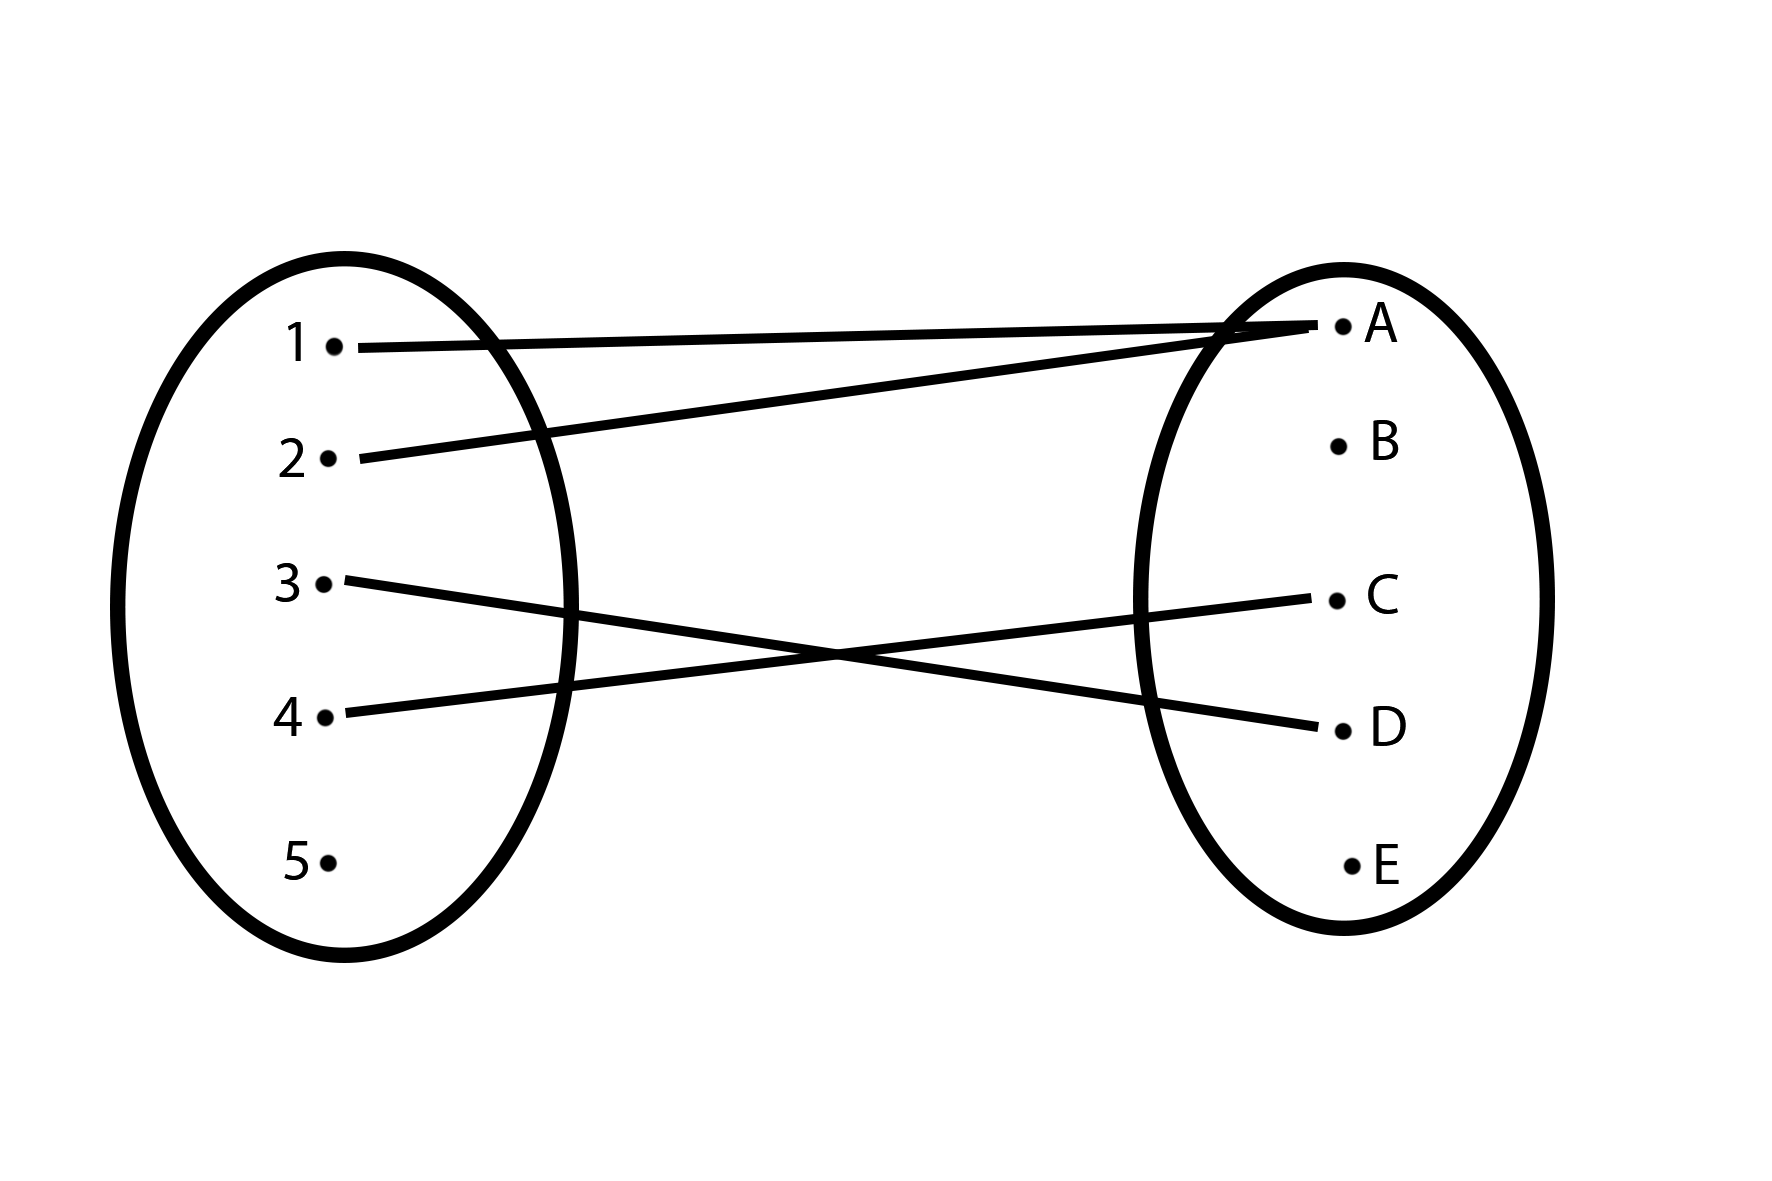
\includegraphics[width=0.7\textwidth]{images/rechtseindeutig.png}
\caption{Rechtseindeutig, Jedes linke Element hat höchtens ein rechtes Element}
\label{fig:Bild1}
\end{figure}
\end{frame}

%Funktionen
\begin{frame}
\frametitle{Funktionen}

Funktionen sind Relationen, die linkstotal und rechtseindeutig sind
\begin{itemize}
\item Jedes Element der Urmenge ("linke" Menge) wird abgebildet (linkstotal)
\item Für jedes Element gibt es nur einen oder keinen Partner in der Zielmenge (rechtseind.)
\item Auch Funktionen können injektiv und surjektiv sein (Sie sind ja Relationen)
\end{itemize}
\end{frame}

\begin{frame}
\frametitle{Funktionen}

Injektive Funktionen sind zum Beispiel
\begin{itemize}
\item $f_1: \mathbb{N} \rightarrow \mathbb{N}, x \mapsto 2x$
\item $f_2: \mathbb{N} \rightarrow \mathbb{N}, x \mapsto x^2$
\end{itemize}
aber nicht
\begin{itemize}
\item $f_3: \mathbb{Z} \rightarrow \mathbb{Z}, x \mapsto x^2$ %f(-1) = f(1)
\end{itemize}
\end{frame}

\begin{frame}
\frametitle{Funktionen}

Surjektive Funktionen sind zum Beispiel
\begin{itemize}
\item $f_1: \mathbb{R} \rightarrow \mathbb{R}, x \mapsto 2x + 1$
\item $f_2: \mathbb{R} \rightarrow [0, \infty ), x \mapsto x^2$
\end{itemize}
aber nicht
\begin{itemize}
\item $f_3: \mathbb{Z} \rightarrow \mathbb{Z}, x \mapsto x^2$ %f(-1) = f(1) Parabel
\end{itemize}
\end{frame}

\begin{frame}
\frametitle{Aufgabe}

Ist die Funktion\\
$f_1: \mathbb{R} \rightarrow \mathbb{R}, x \mapsto x^3$\\
surjektiv bzw. injektiv?\\
\textit{Surjektiv, da mit $x^3$ jede reelle Zahl getroffen werden kann.\\
Injektiv, da kein x in der Zielmenge doppelt getroffen wird ($x^3$ ist für positive x positiv und für negative x negativ)}\\
\ \\
Und wieso ist\\
$f_3: \mathbb{Z} \rightarrow \mathbb{Z}, x \mapsto x^2$\\
weder injektiv noch surjektiv? Beweise mit je einem Gegenbeispiel.\\
\textit{Nicht injektiv, da $f_3(2) = f_3(-2) = 4$. Nicht surjektiv, da -1 nicht getroffen wird.}
\end{frame}

\end{document}
